\section{Solidity Program}
\begin{lstlisting}[language=solidity]{MyFirstContract.sol}
pragma solidity ^0.5.0;

// Create a new Contract
contract MyFirstContract {
	// Declare balance as a uint (256 bit unsigned int) 
	uint balance;

	// View function getBalance - View functions promise to not make any changes to state of contract 
	// Return Value Type (uint) 
	function getBalance() public view returns (uint) {
		return balance;
	}

	// constructor sets balance 
	constructor() public {
		balance = 100;
	}
}
\end{lstlisting}

\begin{lstlisting}[language=solidity]{3\_deploy\_contracts.js}
const MyFirstContract = artifacts.require("./MyFirstContract.sol");

// Export the deployer of  MyFirstContract 
module.exports = function(deployer) {
	// Deploy the MyFirstContract on Network
	deployer.deploy(MyFirstContract);
}
\end{lstlisting}

\begin{lstlisting}[language=solidity]{MyFirstContractTest.js}
const MyFirstContract = artifacts.require("MyFirstContract") 

contract('MyFirstContract', () => {
	it("Should always return 100 when getBalance() is called.", async () => {
		const firstContractInstance = await MyFirstContract.deployed()
		const balance = await firstContractInstance.getBalance()
		assert.equal(balance, 100,
			"Oops! Default balance wasn't 100");
		
	})
})
\end{lstlisting}
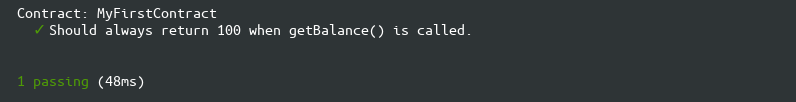
\includegraphics[scale=0.5]{test.png}
\begin{lstlisting}[language=solidity]{truffle-config.js}
module.exports = {
  networks: {
    // Useful for testing. The `development` name is special - truffle uses it by default
    // if it's defined here and no other network is specified at the command line.
    // You should run a client (like ganache-cli, geth or parity) in a separate terminal
    // tab if you use this network and you must also set the `host`, `port` and `network_id`
    // options below to some value.
    //
		 development: {
			host: "127.0.0.1",     // Localhost (default: none)
			port: 8545,            // Standard Ethereum port (default: none)
			network_id: "*",       // Any network (default: none)
		 },

  },

  // Set default mocha options here, use special reporters etc.
  mocha: {
  },

  // Configure your compilers
  compilers: {
    solc: {
    }
  }
}
\end{lstlisting}
